% Wersja z 10 października 2014 r.
\documentclass[11pt,wide]{mwart}
%%%%%%%%%%%%%%%%%%%%%%%%%%%%
%
% Styl dokumentu   : 'mwart'.
% Rozmiar czcionki : '11pt' (domyślnie '10pt', można u¿ywaæ tak¿e czcionki '12pt').
% Numeracja wzorów : po lewej stronie - 'leqno'.
%
%
%%%%%%%%%%%%%%%%%%%%%%%%%%%%%%%%%%%%%%%%%%%%%%%%%%%%%%%%%%%%%%%%%%%%%%%%%%%%%%
% kodowanie latin2 (Linux), cp1250 (Windows)
\usepackage[T1]{fontenc}
\usepackage[utf8]{inputenc}
\usepackage[polish]{babel}
%\usepackage[cp1250]{inputenc}  % Polskie literki...
%\usepackage[OT4,plmath]{polski}% Polskie tytuły, data, bibliografia, itp.

\usepackage{graphicx} 
\usepackage{caption}
\usepackage{subcaption}
\usepackage{epstopdf}

\usepackage{amsmath,amssymb,amsfonts,amsthm,mathtools}
                             

\usepackage{bbm}              
\usepackage{hyperref}
\usepackage{url}

\usepackage{graphicx}
% grafika dodawana z folderu z programem
\graphicspath{ {./../prog/wykresy} }

%\usepackage{comment}   

\raggedbottom

%%%%%%%%%%%%%%%%%%%%%%%%%%%%%%%%%%%%%%%%%%%%%%%%%%%%%%%%%%%%%%%%%%%%%%%%%%%%%%

\date{Wrocław, \today}
\title{\LARGE\textbf{Sprawozdanie z przedmiotu Analiza Numeryczna (M)\\Zadnie 1.4}}
\author{Wojciech Pokój, 324526}

\newtheorem{tw}{Twierdzenie}
\newtheorem{alg}{Algorytm}

\begin{document}
\maketitle                
\thispagestyle{empty}     
\tableofcontents    
%%%%% =========== \begin{samepage} \end{samepage}

\section{Wprowadzenie}

W 1734 roku słynny matematyk Leonhard Euler w swojej pracy zatytułowanej \textit{"De Progressionibus harmonicis observationes"} po raz pierwszy zaproponował stałą, wyrażoną wzorem:

\begin{equation}
\gamma_{n} = (\sum_{k=1}^{n}\frac{1}{k} - \ln{n})
\end{equation}

\begin{equation}
\gamma = \lim_{n \to \infty} \gamma_{n} \approx 0.57721...
\end{equation}

Niedługo później tą stałą nazwano \textit{stałą Euler'a}.
Jej pierwsze przybliżenie zostało obliczone z dokładnością do 5 cyfr znaczących, a na przestrzeni czasu zostały wyznaczone coraz dokładniejsze przybliżenia. Obecnie najprecyzyjniejsze
składa się z 600 milionów cyfr. Do teraz jednak nie zostało pokazane czy ta stała jest niewymierna i czy jest transcendentalna i jest to jeden z ważniejszych problemów we współczesnej matematyce.

Jak się okazuje wyrazy ciągu wyznaczającego tą stałą dla odpowiednio dużego n można przybliżyć używając wzoru:

\begin{equation}
\gamma_{n} - \gamma \approx cn^{-d}, d > 0
\end{equation}

W tej pracy chciałbym doświadczalnie wyznaczyć takie wartości $ d $ oraz $ c $ żeby ciąg $cn^{-d}$ najdokładniej możliwie wyznaczał wyrazy ciągu $\gamma_{n} - \gamma$. Obliczenia będę prowadził liczbach 
zmiennopozycyjnych o podwójnej precyzji (\textit{double}).


\section{Metoda obliczania}

Korzystając z faktu, że logarytm dwójkowy jest funckją różnowartościową i monotonicznie rosnącą, wejściowe równanie jest równoważne:

\begin{equation}
\log(\gamma_{n} - \gamma) \approx \log{cn^{-d}} = \log{c} + -d\log{n}
\end{equation}

Z kolei po wykonaniu podstawienia $[x/\log(n)]$:

\begin{equation}
\log(\gamma_{2^{x}} - \gamma) \approx \log{c} + -dx
\end{equation}

Do przybliżenia wartości $\log{c}$ oraz $-d$ posłużę się liniowym równaniem regresowym dla wybranych wartości $x$.
Równanie to służy do wyznaczenia wpółczynników funckji liniowej najlepiej odzwierciedlającej wykres dla wybranych punktów.
W szczególności interesuje mnie znaleznienie $a$ oraz $b$ dla których funkcja (6) (gdzie $x_i$ oraz $y_i$ to wybrane punkty wykresu) będzie zwracała najmniejszą wartość.

\begin{equation}
f(a, b) = \sum_{i = 1}^{n} ( ax_i + b - y_i)^2
\end{equation}

Wyznaczenia tych wartości można efektywnie wykonać poprzez wyprowadzenia pochodnych częściowych funcji (6) względem zmiennych $a$ oraz $b$ oraz przyrównanie ich do zera.
W szczególności do rozwiązania jest następujący układ równań:

\begin{equation}
f_a(a, b) = \sum_{i = 1}^{n} ( ax_i + b - y_i)x_i = 0
\end{equation}
\begin{equation}
f_b(a, b) = \sum_{i = 1}^{n} ( ax_i + b - y_i) = 0
\end{equation}


Czyli interesujące nas rozwiązanie to rowiązanie układu rówanań:

\begin{equation}
\begin{cases}

a\sum_{i = 0}^n x_i^2 + b\sum_{i=0}^n x_i = \sum_{i = 0}^n x_i y_i \\
a\sum_{i = 0}^n x_i + b\sum_{i = 0}^n 1 = \sum_{i = 0} ^n y_i

\end{cases}
\end{equation}

Dalej ten układ równań jest równoważny równaniu:

\begin{equation}
\begin{bmatrix} \sum_{i = 0}^n 1 & \sum_{i = 0}^n x_i \\ \sum_{i = 0}^n x_i & \sum_{i = 0}^n x_i^2 \end{bmatrix}
\begin{bmatrix} b \\ a \end{bmatrix}
=
\begin{bmatrix} \sum_{i = 0}^n x_i \\ \sum_{i = 0}^n x_i y_i \end{bmatrix}
\end{equation}

Niech X oraz Y będą następtującymi macierzami:

\begin{equation}
X = \begin{bmatrix} 1 & x_1 \\ 1 & x_2 \\ \vdots & \vdots \\ 1 & x_n \end{bmatrix}
Y = \begin{bmatrix} y_1 \\ y_2 \\ \vdots \\ y_n \end{bmatrix}
\end{equation}

Zauważmy, że:

\begin{equation}
X^T X = \begin{bmatrix} 1 & 1 & \dots & 1 \\ x_1 & x_2 & \dots & x_n \end{bmatrix}
\begin{bmatrix} 1 & x_1 \\ 1 & x_2 \\ \vdots & \vdots \\ 1 & x_n \end{bmatrix}
= \begin{bmatrix} \sum_{i = 0}^n 1 & \sum_{i = 0}^n x_i \\ \sum_{i = 0}^n x_i & \sum_{i = 0}^n x_i^2 \end{bmatrix}
\end{equation}

\begin{equation}
X^T Y = \begin{bmatrix} 1 & 1 & \dots & 1 \\ x_1 & x_2 & \dots & x_n \end{bmatrix}
\begin{bmatrix} y_1 \\ y_2 \\ \vdots \\ y_n \end{bmatrix} 
= \begin{bmatrix} \sum_{i = 0}^n x_i \\ \sum_{i = 0}^n x_i y_i \end{bmatrix}
\end{equation}

Zatem wyjściowe równanie dalej redukuje się do postaci:

\begin{equation}
X^T X \begin{bmatrix} b \\ a \end{bmatrix} = X^T Y
\end{equation}

I w końcu do równania:

\begin{equation}
\begin{bmatrix} b \\ a \end{bmatrix} = (X^T X)^{-1} X^T Y
\end{equation}

Tak wyprowadzone równanie posłuży mi do wyzanczenia doświadczalnie stałych $c$ oraz $d$.
Początkowy zbiór $x$-ów (argumentów) ograniczę do zbioru:

\begin{equation}
X = \{ x \in N \ |\  \exists g, h \wedge 1 \le g < 10 \wedge 3 \le h < 5 \wedge n = g*10^{h}\}
\end{equation}

i będę go dopasowywać jeśli się okaże niewystarczający




\section{Wyniki}
% [0.49992305796413217 0.9999873486851487; 0.49648351153988485 0.9988178127930641; 0.49936793133630974 0.9998409941021603; 0.49991530047909666 0.9999834155495929; 0.49999106704057744 0.9999985986202838; 0.500147801151194 1.0000071387531007

\begin{samepage}

Dla tak ustalonego zbioru argumentów $X$ obliczone $c$ oraz $d$ wynoszą:
\begin{equation}
\begin{align}
c = 0.49992305796413217\\
d = 0.9999873486851487
\end{align}
\end{equation}

\end{samepage}

\begin{samepage}
Błąd względny i bezwględny przybliżenia zawierały się w przedziałach:
\begin{equation}
\begin{align}
0.0000019730 \le | \gamma_n - \gamma  - cn^{-d}| \le 0.0001445246\\
0.0000001060 \le | \frac{\gamma_n - \gamma  - cn^{-d}}{\gamma_n - \gamma} | \le 0.0000131793
\end{align}
\end{equation}
\end{samepage}

\begin{samepage}
Porównanie ciągu $\gamma_n - \gamma$ oraz funkcji $cn^{-d}$ przedstawia wykres:

\vspace{1cm}
\centerline{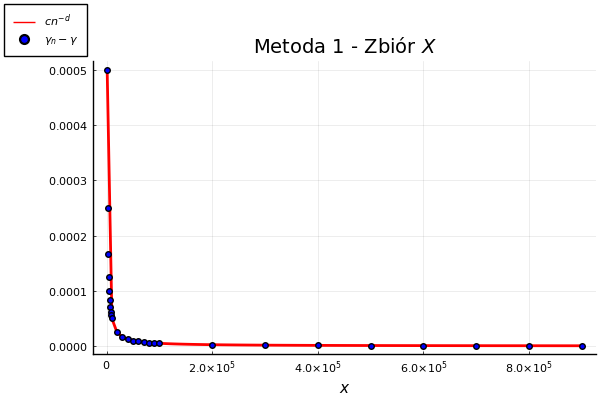
\includegraphics[scale=0.8]{chart1_1}}
\vspace{1cm}

\end{samepage}

Jak widać na wykresie, ta funkcja kształtem bardzo dobrze oddaje ciąg $\gamma_n - \gamma$. 
Przetestuję tą samą metodę na kilku innych zbiorach i porównam wyniki z wynikami dla pierwotnego zbioru $X$.

\begin{samepage}
Niech $X_i$ będzie zbiorem:
\begin{equation}
X_i = \{n \in \mathbb{N} | \exists a \in \mathbb{N} \wedge a \le 33 \wedge n = 3a + 10^i\}
\end{equation}
\end{samepage}

\begin{samepage}
Wyniki metody regresji dla $X, X_2, X_3, X_4, X_5, X_6$ są następujące:

\begin{center}
\begin{tabular}{||c c c c c c c||} 
 \hline
	    & C         & D         & $min_{BB}$        & $max_{BB}$       & $min_{BW}$        & $max_{BW}$        \\ [0.5ex] 
 $X$    & 0.4999230 & 0.9999873 & 1.060e-07 & 1.318e-05 & 1.973e-06 & 1.445e-04 \\ 
 $X_2$  & 0.4964835 & 0.9988178 & 1.281e-07 & 1.026e-05 & 1.083e-06 & 7.847e-05 \\
 $X_3$  & 0.4993679 & 0.9998409 & 1.843e-10 & 1.544e-08 & 2.041e-09 & 1.693e-07 \\
 $X_4$  & 0.4999153 & 0.9999834 & 1.599e-10 & 1.817e-10 & 2.286e-09 & 2.597e-09 \\
 $X_5$  & 0.4999910 & 0.9999985 & 5.014e-09 & 5.056e-09 & 8.830e-08 & 8.904e-08 \\ 
 $X_6$  & 0.5001478 & 1.0000071 & 1.358e-05 & 1.358e-05 & 2.842e-04 & 2.842e-04 \\ [1ex]
 \hline
\end{tabular}
\newline
\small{Kolejne kolumny od lewej: Obliczone wartości $c$ oraz $d$, minimalny i maksymalny błąd bezwzględny dla danego przedziału, minimlany i maksymalny błąd względny.}

\end{center}

\end{samepage}
Z powyższych wyników można wyciągnąć kilka wniosków:

\begin{itemize}

\item Krótsze ale bardziej zagęszczone zbiory argumentów przybliżają lepiej wartości $c$ oraz $d$ w danych przydziałach.

\item Dla wartości rzędu $10^4$ wartości $c$ i $d$ są jakościowo najlepiej dobrane (najmniejsze błędy maksymalne).

\begin{samepage}
\item Dla wartości rzędu $10^6$ powstają duże błędy względne i bezwględne. Wynikać to może ze zjawiska utraty cyfr znaczących przy wykonywaniu odejmowania $\gamma_n - \gamma$.
	Dla zbioru $X_6$ obliczone wartości trzeba traktować ostrożnie. Problem dobitnie widać na wykresie dla przedziału $X_6$:
	
\vspace{1cm}
\centerline{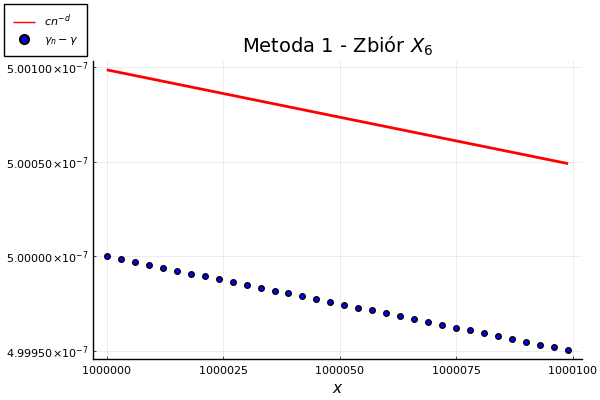
\includegraphics[scale=0.8]{chart1_6}}
\vspace{1cm}

\end{samepage}
	
\item Pomijając wątpliwej jakości wyniki dla zbioru $X_6$ możemy wywnioskować, że liczby $c$ i $d$ dążą do:
	\begin{equation}
		c \to \frac{1}{2}; \quad d \to 1
	\end{equation}

\end{itemize}



\section{Metoda druga}

Sprawdzenie otrzymach wyników wykonam inną metodą. Zauważmy, że stałe $c$ oraz $d$ rozważanego ciąg $cn^{-d}$ można potraktować jako stałą asymptotyczną zbieżności
oraz wykładnik zbiezności ciągu $\gamma_n$ o granicy $\gamma$. 

Niech $e_n$ będzie ciągiem błędów kolejnych przybliżeń ciągu $\gamma_n$, tj. $e_n = \gamma_n - \gamma$\\
\begin{samepage}
Dla $n \to \infty$ mamy:

\begin{equation}
|e_{n+1}| \approx c|e_n|^d 
\end{equation}
\begin{equation}
|e_{n}| \approx c|e_{n-1}|^d
\end{equation}

\end{samepage}

\begin{samepage}
Stąd: 

\begin{equation}
\frac{|e_{n+1}|}{|e_{n}|} \approx \frac{c|e_{n}|^d}{c|e_{n-1}|} \approx \mid \frac{e_n}{e_{n-1}} \mid^d
\end{equation}
\end{samepage}


\begin{samepage}
Rozwiązując dla $d$:

\begin{equation}
d \approx \frac{log(e_{n+1} / e_n)}{log(e_{n} / e_{n-1})}
\end{equation}

Ponieważ granica ciągu $\gamma_n$ jest znana nie trzeba stosować dalszych przekształceń dla tej metody

\end{samepage}


\section{Wyniki drugiej metody}

Drugą metodę, podobnie jak pierwszą, przetestowałem na kilku przedziałach, zdefiniowanych następująco:
$$
A_1 = \{10^3, 10^3+20, 10^3+40, \dots, 10^3+980\}
$$
$$
A_2 = \{10^4, 10^4+20, 10^4+40, \dots, 10^4+980\}
$$
$$
A_3 = \{10^6, 10^6+20, 10^6+40, \dots, 10^6+980\}
$$


Wyniki dla przedziału $A_1$ zawiera poniższy wykres:

\vspace{1cm}
\centerline{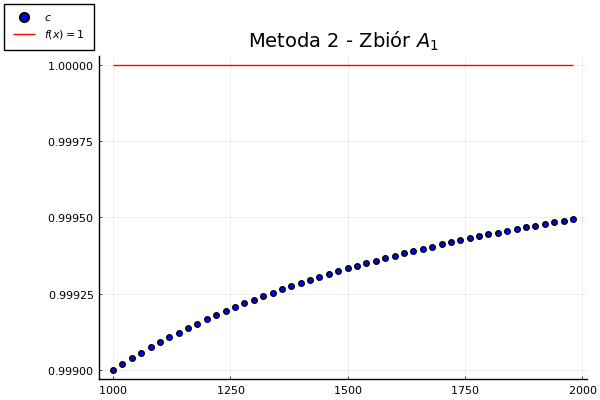
\includegraphics[scale=0.8]{chart2_1}}
\vspace{1cm}

Jak się okazuje kolejne przybliżenia wykładnika zbiezności $d$ zachowują się podobnie jak w pierwszej metodzie,
t.j. tworzą ciąg rosnący i nie przekraczają wartości 1.
Pojawiają się już jednak pewne problemy dla argumentów rzędu $10^4$.
Wykres dla zbioru $A_2$ nie jest tak równy jak dla poprzedniego zbioru.

\vspace{1cm}
\centerline{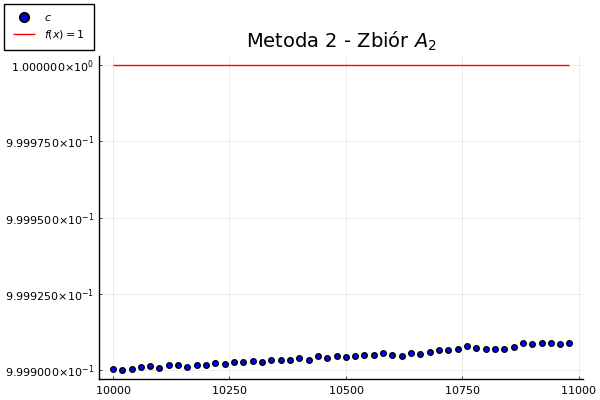
\includegraphics[scale=0.8]{chart2_2}}
\vspace{1cm}

Na tym wykresie gołym okiem widać że kolejne przybliżenia są coraz gorszej jakości. Wartości przestają formować ładną krzywą jak w poprzednim przykładzie.
Pomimo tego dalej możemy mówić o potencjalnej zbieżności przybliżeń do wartości 1.
Dla przypomnienia dla tego rzędu wartości metoda regresji liniowej zwróciła najlepsze lokalne przybliżenie wartości $d$ oraz $c$.

Dla ostatniego zbioru wykres jest następujący:

\vspace{1cm}
\centerline{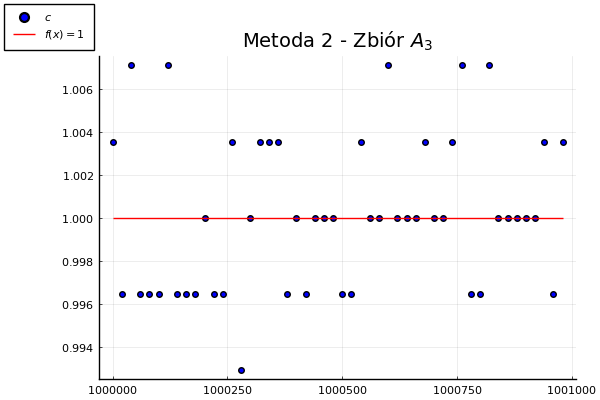
\includegraphics[scale=0.8]{chart2_3}}
\vspace{1cm}

Wartości bardzo chaotycznie oscylują wokół prostej $f(x) = 1$.
Powodem tego może być fakt że wzór na przybliżenie $d$ wymaga dzielenia kolejnych wyrazów ciągu $e_n$ które liniowo zbiegają do zera. W połączeniu ze zjawiskiem utraty cyfr znaczących
powstały błąd kumuluje się i daje nieprzewidywalne wartości. Jest to pewien problem okupiony korzystaniem z arytmetyki 64-bitowej. Lepsze wyniki dla tego rzędu wartości będą trudne do uzyskania.

\section{Porównanie metod}

W ostatnim rozdziale chciałbym się pochylić nad zagadnieniem porówania obu metod.
Interesuje mnie kilka zagadnień:
\begin{itemize}
\item szybkość zbiegania do przewidywanego wykładnika zbiezności poszczególnych metod,
\item odporność na zjawisko utraty cyfr zanczących.
\end{itemize}

Porównanie metod dla poszczególnych wartości wykonam przez wyliczanie 3 kolejnych wyrazów ciągu $e_n$ i zaaplikowaniu ich do obu metod.
Porównanie wykonam na przedziałach $A_1$, $A_2$ i $A_3$ zdefiniowanych jak w poprzednim rozdziale

Wyniki są następujące:

\vspace{1cm}
\centerline{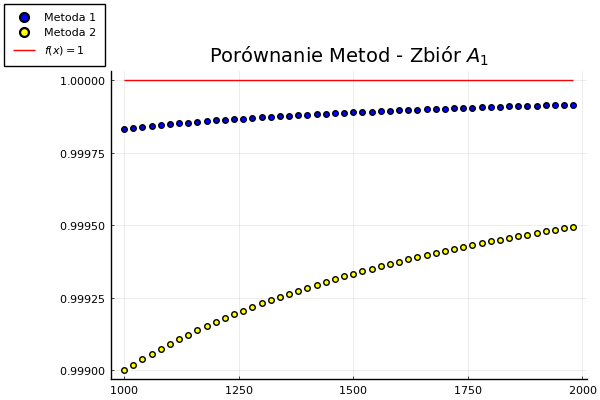
\includegraphics[scale=0.8]{chart3_1}}
\vspace{1cm}
\centerline{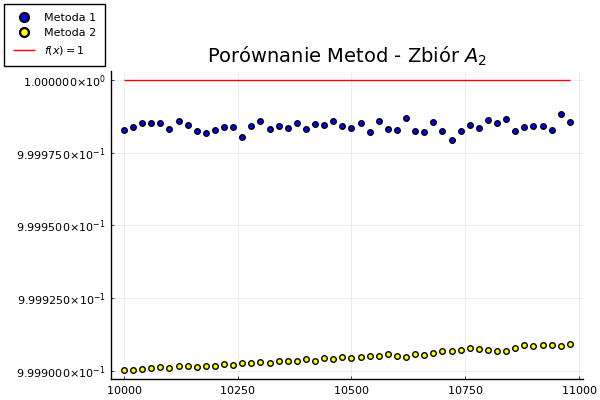
\includegraphics[scale=0.8]{chart3_2}}
\vspace{1cm}
\centerline{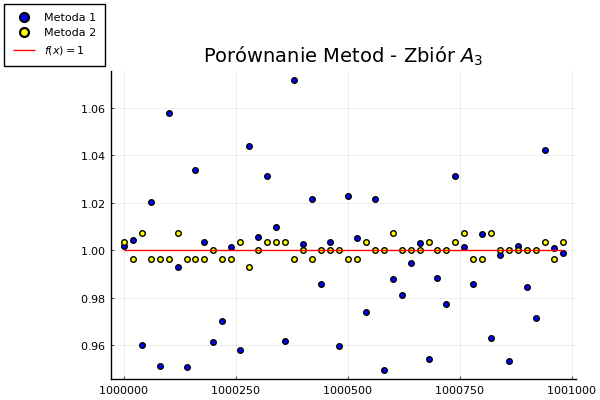
\includegraphics[scale=0.8]{chart3_3}}
\vspace{1cm}

Można zauważyć że obie metody posiadają pewne zalety i wady.
Mianowicie, metoda regresji liniowej dużo szybciej zbiega do oczekiwanej wartości, ale również dużo szybciej pada ofiarą kumulującego się błędu ciągu $e_n$.
Z kolei druga metoda zachowuje się zgoła odwrotnie, zbiega wolniej, ale wartości są mniej rozrzucone po wykresie.
Widać to dobrze dla przedziału $A_3$ gdzie metoda aproksymacji wykładnika ściślej przylega do funkcji $f(x) = 1$ niż metoda regresji liniowej.

Pomimo tego podziału zalet między metodami trzeba zauważyć że metoda regresji liniowej jest bardziej uniwersalna i co najważniejsze,
u podstaw tej metody leży problem minimalizacji odchylenia standardowego, więc dodanie punktów dla których znamy dokładne wartości pomaga
poprawić wyniki tej metody. Jednak jest to okupione faktem, że żeby z tej własności skorzystać musimy wiedzieć coś więcej o badnym ciągu, co nie zawsze jest możliwe.

\section{Literatura}

\begin{enumerate}
	\item  D. Kincaid, W. Cheney, \textit{Analiza numeryczna}, WNT, 2005.
\end{enumerate}


\vspace{1cm}
\end{document}






















